\documentclass[fleqn,10pt]{wlscirep}
\usepackage[utf8]{inputenc}
\usepackage{array}
\usepackage{pdflscape}
\usepackage{longtable}
\usepackage{threeparttable}
\usepackage[table]{xcolor}
\usepackage{tcolorbox}
\usepackage{xspace}
\usepackage{xcolor}
\usepackage{graphicx}
\definecolor{heatmap1}{RGB}{8,48,107}    % Dark Blue (High value)
\definecolor{heatmap2}{RGB}{33,113,181}  % Medium Blue
\definecolor{heatmap3}{RGB}{66,146,198}  % Light Blue
\definecolor{heatmap4}{RGB}{107,174,214} % Lighter Blue
\definecolor{heatmap5}{RGB}{198,219,239} % Very Light Blue
\definecolor{heatmap6}{RGB}{237,248,251} % Almost White

%Redline version
\newcommand{\edit}[1]{\textcolor{red}{#1}}
\newcommand{\goedit}[1]{\textcolor{black}{#1}}

\def\ourmetric{\texttt{Spurious Rate}\xspace}


\tcbset{
  palebluebox/.style={
    enhanced jigsaw,     % use the jigsaw engine for flexible breaking
    breakable,           % allow the box to split across pages
    colback=gray!10!white,
    colframe=gray!30!white,
    boxrule=0pt,
    sharp corners,
    width=\textwidth,
    before skip=10pt,
    after skip=10pt,
    left=8pt, right=8pt, top=3pt, bottom=3pt,
  }
}

\usepackage[T1]{fontenc}
\usepackage{makecell}
\title{Measuring Physicians and LLM Relevance Alignment in Medical Question Answering}

% \author[]{Anonymous Author(s)}
\author[1,2 *]{Yuexing Hao, Ph.D.}
\author[1]{Kumail Alhamoud, M.S.}
\author[1]{Hyewon Jeong, M.D., M.S.}
\author[1]{Haoran Zhang, M.S.}
\author[1]{Grace Yan, B.S.}
\author[1]{Isha Puri, B.S.}
\author[3]{Philip Torr, Ph.D.}
\author[6]{Mike Schaekermann, Ph.D.}
\author[2]{Saleh Kalantari, Ph.D.}
\author[4,5]{Ariel D. Stern, Ph.D.}
\author[1]{Marzyeh Ghassemi, Ph.D.}

\affil[1]{Massachusetts Institute of Technology, Cambridge, MA, 02139, USA}
\affil[2]{Cornell University, Ithaca, NY, 14850, USA}
\affil[3]{University of Oxford, Oxford, UK}
\affil[4]{Hasso Plattner Institute, Potsdam, Germany}
\affil[5]{University of Potsdam, Potsdam, Germany}
\affil[6]{Independent Researcher}

\affil[*]{Corresponding Author: yuexing@mit.edu}


\begin{abstract}
Large Language Models (LLMs) have demonstrated strong performance on medical question answering (QA) benchmarks, including standardized medical exams. Correct answers alone, however, do not guarantee correct reasoning, as a model can reach the right conclusion while attending to input that a clinician would consider unimportant. In this study we evaluate how physician trainees and LLMs report sentence-level relevance when answering clinical QA items. We obtain annotations on 933 QA pairs from 53 physician trainees, with a subset independently reviewed by 7 board-certified physicians. These annotations label each sentence of the case description as high-relevance, low-relevance, or irrelevant. We then compare these human annotations against LLM-derived relevance labels and measure the effect of restricting the LLM input to the sentences each labeler considers relevant. The average sentence-level concordance between LLMs and the physician trainees' majority vote ranges from 44.9\% to 65.9\%, while the concordance between physician trainees and the board-certified physicians is 72.0\%, indicating a modest but consistent gap. Removing sentences that physician trainees judge as low-relevance or irrelevant increases the accuracy of most LLMs on the four source datasets, and similar but more modest gains are observed when each LLM filters its own input or the input of another model. These results suggest that current LLMs do not consistently prioritize the same case information as physician trainees, and that relevance-aware filtering can potentially be a useful aspect of model reasoning. The findings are based on multiple-choice exam questions and should be interpreted as an evaluation step, rather than direct evidence of readiness for clinical deployment.
\end{abstract}

\begin{document}

\flushbottom
\maketitle

\section{Main}

Large language models (LLMs) have shown strong performance on medical diagnostic tasks \cite{de2025we}, with systems such as GPT-4 \cite{openai_gpt-4_2024} and MedPaLM \cite{singhal2023large} outperforming human averages on standardized medical examinations \cite{cabral_clinical_2024, mcduff_towards_2025, liu2025generalist, holmes2025radonc, van2024adapted}. Multiple LLM companies including OpenAI and Anthropic have launched specific HIPAA-compliant LLMs targeting the healthcare market. However, the high performance of these LLMs on exam-style datasets may overstate their generalizability~\cite{li_mediq_2024, hao2025large, deng-etal-2024-investigating}, due to multiple-choice exam tasks not reflecting the complexity of real-world use cases, among other issues \cite{xia_cares_2024}. In human-facing settings, it is crucial to understand how models filter and prioritize relevant information \cite{park_does_2015}.

Estimation of contextual relevance is a critical aspect in many applications \cite{KonopaskyArtinoBattistaOhmerHemmerTorreRamanivanMerrienboerTeunissenMcBeeRatcliffeDurning+2020+257+264, sayres2025towards, hao2024outcome}. Techniques such as semantic entropy \cite{farquhar_detecting_2024}, influence functions \cite{choe_what_2024}, context attribution \cite{cohen-wang_learning_2025, liuattribot2024}, and evidence inference \cite{deyoung_eraser_2020} have been employed to assess which elements within a context hold the most importance. Despite these efforts, existing relevance estimations are often imprecise and noisy, with models sometimes producing misleading or overly confident assessments that deviate from human judgment \cite{es_ragas_2024}. Even when estimations appear less noisy, model-generated relevance labels may not concord with those of human experts. This gap is particularly concerning in human-facing domains where alignment with expert judgment is necessary \cite{zhao_moverscore_2019, schuler_context_2025}. 

Models may depend on input features that a clinician would not treat as informative \cite{adam2022mitigating}. Prior work has shown that restricting inputs to relevant content can reduce distraction, streamline evidence integration, and lower memory requirements \cite{khattab_baleen_2021, chuang_selfcite_2025, lu_learn_2022, bucinca_trust_2021}. Small, clinically unimportant perturbations of medical questions have also been shown to produce statistically significant shifts in model treatment recommendations \cite{gourabathina2025medium}. To date, however, little work has examined whether models and physicians agree on which case information is worth attending to, or whether concentrating models on such content measurably improves downstream answers.

Characterizing the extent to which LLMs attend to the same input sentences that clinicians treat as informative is a useful step toward understanding how these models derive their answers \cite{strong_chatbot_2023, katz_gpt_2024}. Such comparisons can complement accuracy based evaluation by flagging cases where a correct answer is accompanied by reliance on sentences that clinicians would not regard as decisive \cite{chiang_can_2023, McCoy_NEJM_SCTBenchmark}. Alignment between model attributed and clinician identified evidence has also been proposed as one of several factors relevant to clinician trust in diagnostic AI tools \cite{huang2025trustworthiness, huang2026probellm}. Restricting LLMs to sentences that clinicians judge highly relevant provides an auditing lens to evaluate the extent to which model predictions depend on content that humans consider peripheral \cite{zhou_explainable_2025, wu_medreason_2025, bansal_does_2021}. Such dependencies do not always reduce benchmark accuracy, but they can complicate the interpretation of benchmark performance.

A related concern is that LLMs may be trained on data that overlap with public medical benchmarks. Relevance-aware filtering does not by itself distinguish memorization from genuine reasoning, but it offers one additional axis along which such effects can be examined. In our setting the four source datasets span release dates from 2020 to 2025, so the potential for training set contamination varies across subsets; we treat this as a confound rather than as a controlled variable.

To study how physician trainees and LLMs rate the relevance of contextual input in patient cases, we curate a novel dataset called \emph{MedPAIR} (\underline{Med}ical \underline{P}hysician trainee and \underline{AI} \underline{R}elevance) which pairs sentence-level relevance annotations from physician trainees with LLM-derived relevance labels on the same QA items. We then use this dataset to run an empirical study of relevance misalignment. Three research questions organize the study. RQ1: To what extent do physician trainees and current LLMs agree on which sentences of a clinical vignette matter for answering its question? RQ2: Does restricting an LLM's input to sentences that physician trainees label as highly relevant change downstream answer accuracy, and how should such changes be interpreted given potential confounds? RQ3: Can an LLM's own sentence-level relevance scores drive comparable filtering effects using a two-stage process, so that the approach does not depend on human annotation? Medical QA datasets are a primary method of evaluating LLM performance in clinical tasks \cite{pal_medmcqa_2022, zhang_survey_2024, jin_rjua-meddqa_2024, soni_radqa_2022}, yet existing resources primarily score final answers and do not track which parts of the case the model or the human relied on for obtaining that answer \cite{toma_clinical_2023, adlakha_evaluating_2024, bedi2026medhelm}. Recent work on explanation-generation and qualitative reasoning analyses instead focuses on the reasoning produced after the input context has already been interpreted \cite{khandekar2024medcalc}.
%To improve our understanding of what context in the QA that LLM used for answering, we first need a comparison study between domain experts and LLM's relevance labels and measure its alignment. % Recent work has argued that the absence of expert-annotated reasoning data limits the development of reliable models  \cite{zhou_explainable_2025, tang_medagents_2024}. 

We collect sentence-level relevance labels on 933 samples drawn from four source datasets: \textit{Massive Multitask Language Understanding}  (MMLU)-precision medicine (192 QAs) \cite{hendrycks_measuring_2021}, \textit{Medbullets} (160 QAs), \textit{JAMA Clinical Challenge Dataset} (295 QAs) \cite{chen_benchmarking_2025}, and \textit{MedXpertQA} (286 QAs) \cite{zuo_medxpertqa_2025}. These labels are produced by 53 physician trainees, and an additional 7 physician experts spot-check the labels to confirm their reliability.
For the LLM-generated relevancy labels, two distinct approaches are used. First, we prompt all of the studied LLMs (GPT-4o \cite{hurst2024gpt}, GPT-5 \cite{singh2025openai}, MedGemma-27B \cite{sellergren2025medgemma}, Qwen2.5-14B-Instruct, Qwen2.5-72B-Instruct \cite{qwen_qwen25_2025}, and Llama-3.1 70B-Instruct \cite{grattafiori_llama_2024}) to self-report sentence-level input relevance~\cite{choi_identifying_2024, wang-etal-2025-medcite}. Second, we use ContextCite \cite{cohen-wang_contextcite_2024} to retrieve sentence-level relevancy from the four open-source LLMs tested.
%ContextCite is a context attribution framework that reversely maps model outputs to the input sentences which are most responsible for their generation. This approach allows us to quantify the degree of alignment between human and model assessments of contextual importance. 


To address the research questions we first measure sentence-level rating concordance (see the Methods section for more details). The physician experts are found to agree with the physician trainees' majority vote at 72.0\%, while LLM concordance with the physician trainees' majority vote ranges from 44.9\% to 65.9\%. We then examine how restricting the input to the sentences marked as highly relevant affects downstream LLM performance. The results indicate that most of the LLMs gain accuracy after this filtering, both when the filter is derived from physician trainee labels and when it is derived from an LLM. Finally, we quantify a \ourmetric per model, defined as the fraction of originally correct answers that become incorrect once sentences identified by physician trainees as low-relevance or irrelevant are removed. This rate ranges from 5.8\% to 24.8\% in our sample; it is best interpreted as a proxy for the LLMs' reliance on content that physician trainees did not consider decisive, rather than as a direct measure of spurious reasoning. Overall, the study contributes an empirical characterization of how current LLMs and physician trainees diverge on sentence-level relevance in clinical QA, alongside the release of \emph{MedPAIR} as a paired-annotation dataset that enables this analysis as well as potential related work in future studies.  %Our full workflow can be found in Figure \ref{fig:study_design}.

\section{Results}
\subsection{The MedPAIR Dataset and Study Design}

\subsubsection{Medical QA Dataset Construction}
To examine the alignment between physician trainees’ and LLMs’ assessments of relevance, we concentrate on existing QA pairs grounded in specific patient case scenarios, rather than general evidence-based questions. We draw on four source datasets released in different years: \textit{Massive Multitask Language Understanding}  (MMLU)-precision medicine (released September 2020)\cite{hendrycks_measuring_2021}, \textit{Medbullets} (released March 2021), \textit{JAMA Clinical Challenge} (items collected from July 2013 to October 2023)\cite{chen_benchmarking_2025}, and \textit{MedXpertQA} (released January 2025) \cite{zuo_medxpertqa_2025}. The Medbullets and JAMA papers were preprinted in April 2025, and JAMA items require paywall access. The four source datasets have different characteristics; for example, JAMA Clinical Challenge items are usually lengthier and include more extensive details compared to the other three datasets. More extensive characteristics for each dataset are presented in the Supplementary Information. Each source provides multi-sentence patient case descriptions paired with questions (4-option or 10-option multiple-choice) and the associated answers, offering a rich context for relevance annotation. Such patient vignettes are broadly recognized as important training and evaluation documents in the medical and social sciences, and physician responses to clinical vignettes have been shown to predict realized billing behavior in the U.S. Medicare system \cite{cutler_physician_2019}. We obtained approval from the MIT Committee on the Use of Humans as Experimental Subjects (IRB: 2504001610) and preregistered our dataset collection protocol on the Open Science Framework (OSF) \cite{hao_alhamoud_jeong_puri_torr_kalantari_schaekermann_stern_ghassemi_2025}. No personally identifiable patient information was involved in this study.

%Each QA presents a detailed vignette, which is often a long case description covering patient demographic information, symptoms, exam findings, family history, etc. 
%From a combined pool of 4,052 QA pairs, we constructed the final dataset by randomly sampling 250 pairs each from MMLU and Medbullets, and 750 pairs each from JAMA and MedXpertQA, resulting in a curated dataset of 2,000 QA pairs. By pooling these sources, \emph{MedPAIR} covers a wide spectrum of clinical topics and difficulty levels, ensuring that the evaluation is robust across various scenarios from routine to rare conditions. 

\begin{table}[h!]
\centering
\normalsize
\setlength{\tabcolsep}{10pt} 
\begin{tabular}{l|l|c|c|c|c}
\toprule
\textbf{Dataset} & \textbf{Data Source} & \textbf{Total QA} & \textbf{\makecell[c]{Number of\\ Answer Options}} & \textbf{\makecell[c]{Average\\ Sentence Rating}} & \textbf{\makecell[c]{Physician-Labeled Sentences as\\ Low-Relevance or Irrelevant (\%)} }\\
\toprule
\midrule
\textbf{\makecell[l]{MMLU \\{\small(Precision Medicine)}}}  & Medical Textbooks & 192 & 4 & 15.9 {\small(7.0)} & 39.5\% \\\hline
\textbf{\makecell[l]{JAMA \\ Clinical Challenge}}  & Journal Articles & 295 & 4 & 26.8 {\small(8.5)} & 35.0\% \\\hline
\textbf{MedBullets}  & USMLE & 160 & 4 & 21.0 {\small(4.6)} & 40.5\% \\\hline
\textbf{MedXpertQA}  & Licensing Exam & 286 & 10  & 14.9 {\small(5.6)} & 32.8\% \\
\bottomrule
\textbf{Overall}  &   & 933 & 4/10 & 21.3 {\small(8.8)} & 36.1\% \\
\bottomrule
\end{tabular}
\vspace{0.7mm}
\caption{\textbf{Comparative Analysis of Physician Trainee–Annotated \emph{MedPAIR} Dataset Characteristics.} Values in parentheses represent standard deviations.}
\label{tab:comparison_1}
\end{table}


\begin{figure}[h!]
  \centering
  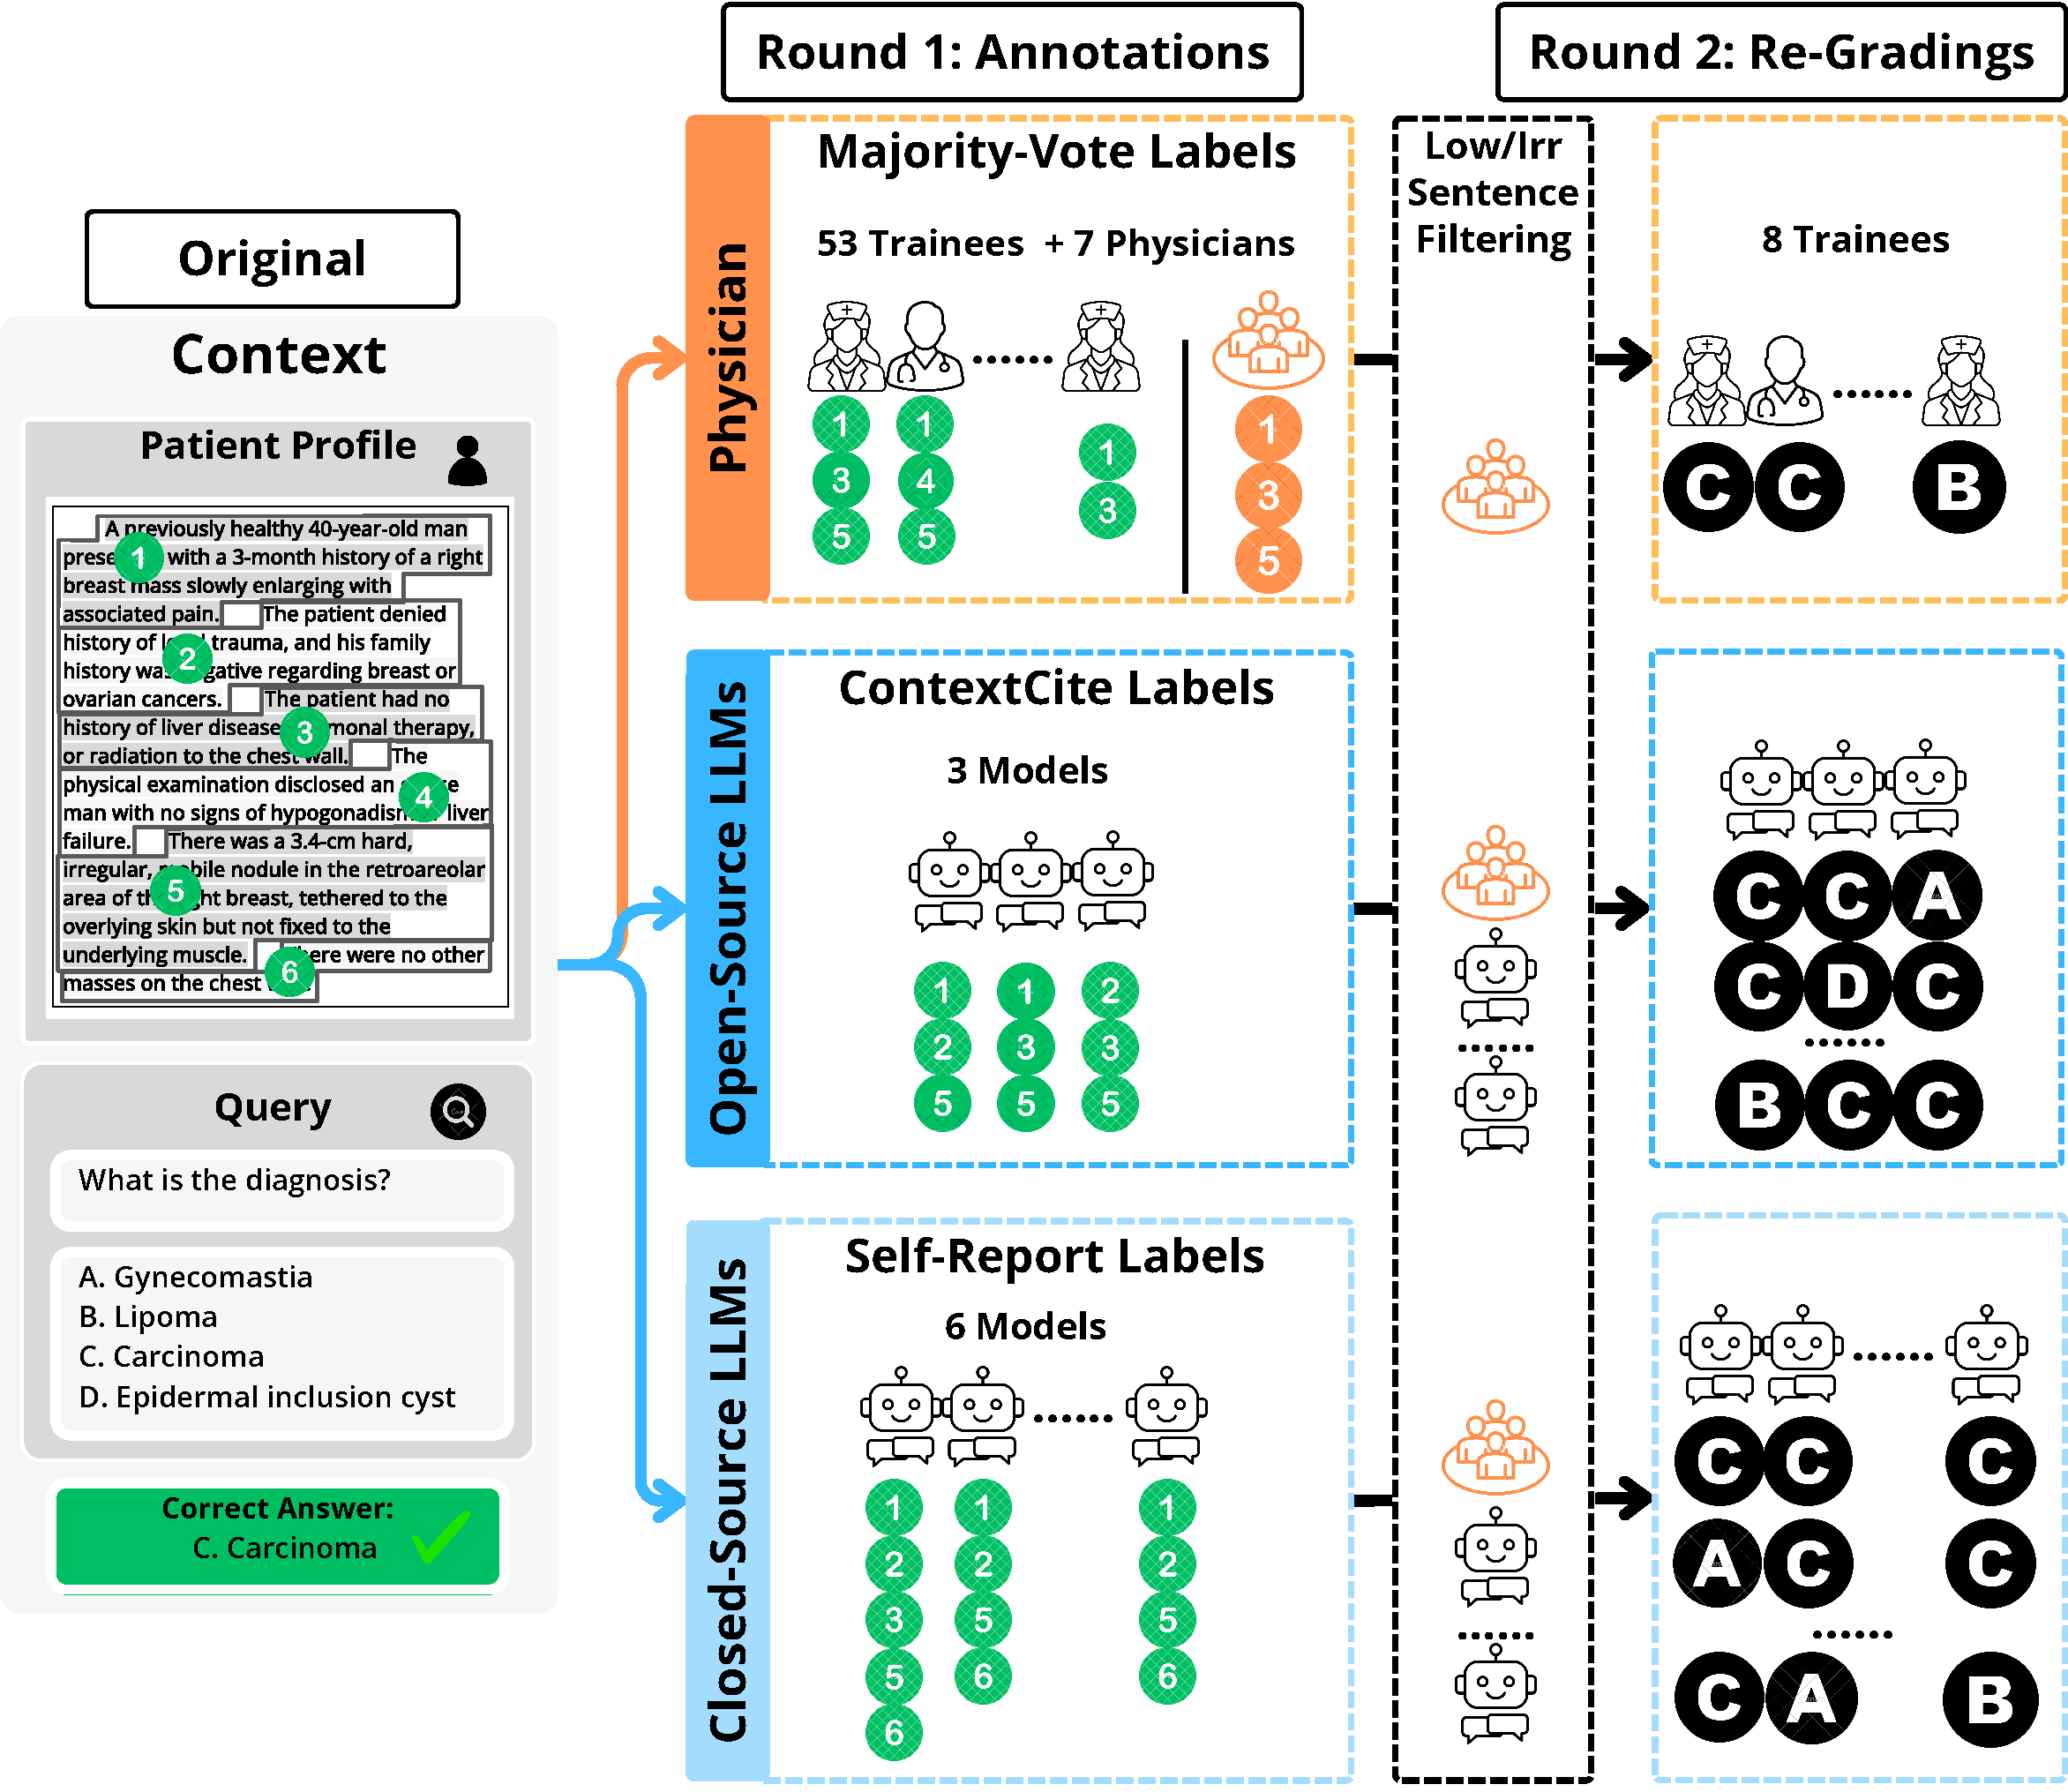
\includegraphics[width=0.95\textwidth]{Figures/MedPAIR-Nature.pdf}
  \caption{\textbf{Study Design.} }
  \label{fig:study_design}
\end{figure}

Across the four datasets, there are 4,052 QA pairs in total. We first remove 2,052 pairs in which the patient profile contains fewer than three sentences. We then exclude 629 pairs that have one or no correct answers, as well as 448 pairs that require information from modalities other than text (e.g., images). This leaves us with a final set of 933 QA pairs that are used in MedPAIR.
Centaur Labs (\url{https://centaur.ai}) is used as the online labeling platform to recruit 52 physician trainees. These participants produce a total of 6,224 sentence labels on the 2,000 QA pairs.
We remove all questions that no PT can answer correctly (448 pairs), leaving us with 933 QA pairs. 
%Only 2,918 labels answer the step 1 classification correctly (Figure \ref{fig:study_design} panel B). 
% We also remove QAs which PT label as containing only highly relevant sentences, as there would be no impact from low or irrelevant sentences removal (104 QA). The final set of QAs is 1,267.
 
%Figure \ref{fig:study_design} shows the \emph{MedPAIR} data curation process.

\subsubsection{Expert Review and Content Analysis of Physician Trainee Labels}

Physician-trainee participants are used in the study due to the logistical difficulties and expense of having board-certified physicians annotate the full dataset. To verify the reliability of the trainee annotations, we use an expert physician review to spot-check a randomly selected subset of the trainee labels. To compare the two groups, we aggregate the trainee labels on each sentence into a single majority vote and compare it to the label assigned by a board-certified physician. The average sentence-level matching rate between the physician trainee majority vote and the reviewing physicians on the items tested is 72.0\% (median 73.7\%, SD 17.7\%, 95\% CI [0.710, 0.730]). A cumulative distribution of these matching rates is presented in the Appendix. We interpret this value as a measure of trainee-physician agreement rather than of trainee accuracy, since the physicians themselves represent a small cohort and inter-physician disagreement is not separately evaluated.

We refer to QA items for which the expert matching rate falls below 20\% as ambiguous cases and retain them in the dataset so that this subgroup can be analyzed separately. Where the downstream analyses in this paper treat the physician trainee majority vote as a reference, this choice is a pragmatic one driven by scale, and the resulting concordance and filtering results should be interpreted against the 72.0\% overall expert-matching average.

% \subsubsection{Qualitative Feedback from Physician}

As a further step, a single board-certified physician is asked to conduct a qualitative comparison of labels that trainees have marked as high- and low-relevance across 30 randomly selected QA pairs. This evaluation indicates that sentences regarded as highly relevant contain more information about anatomical structures and comparative descriptions (e.g., progressive, increased), whereas low-relevance text includes more historical information (e.g., medication, allergy, travel, social) and negative findings (e.g., uncomplicated, noncontributory). %(Table \ref{tab:keyword_readability})

This physician further grouped the low-relevance and irrelevant sentences into four thematic categories, including (1) Redundant clinical details, (2) Negative result that is not essential for the current chief complaint, (3) Low or irrelevant temporal information, and (4) History that provides little relevant clinical information. Further details of this sample case study are presented in the Supplementary Information.

% THIS IS ABOUT WHAT GETS LABELED AS RELEVANT FROM SUBSET, NOT ABOUT THE DATA BEING OKAY TO SUBSET
The trainee relevance labels on all 933 QAs are also compared numerically in terms of words per sentence and perplexity. The highly relevant sentences are found to be consistently longer as well as more uniform in structure, with lower perplexity values and thus greater linguistic predictability. In contrast, irrelevant or low-relevance sentences are shorter on average and have less uniform structures. Further details of this analysis are presented in the Supplementary Material. %There is a clear distinguish between the high and low/irrelevant sentences.

To compare the continuous ContextCite scores produced for the open-source LLMs with the ternary labels assigned by the physician trainees, we map the numerical scores into the ternary scheme. For each QA pair, we let $k$ equal the number of sentences marked as highly relevant by the physician trainees' majority vote. We then order all sentences by their ContextCite scores and assign the top $k$ sentences to the \textit{high relevance} category. A similar process is followed to categorize the remaining ContextCite scores as \textit{low relevance} or \textit{irrelevant} using the corresponding trainee counts. This procedure aligns the LLM and human label distributions per item, which makes concordance directly interpretable in terms of which sentences each source considers most important. Since the total number of sentences placed in each category is held fixed across labelers for a given QA, the resulting concordance rates reflect the ordering produced by each method rather than differences in how many sentences each method would otherwise label as relevant. We therefore treat concordance in this paper as a measure of ranking agreement. The sensitivity of concordance to alternative thresholding choices is discussed in the Supplementary Information. With the ContextCite scores mapped onto the same ternary scheme, we are able to evaluate their correspondence with the physician trainee annotations.

\subsection{Humans and LLMs Often Disagree on Information Relevance (RQ1)}

\begin{figure}[h!]
  \centering
  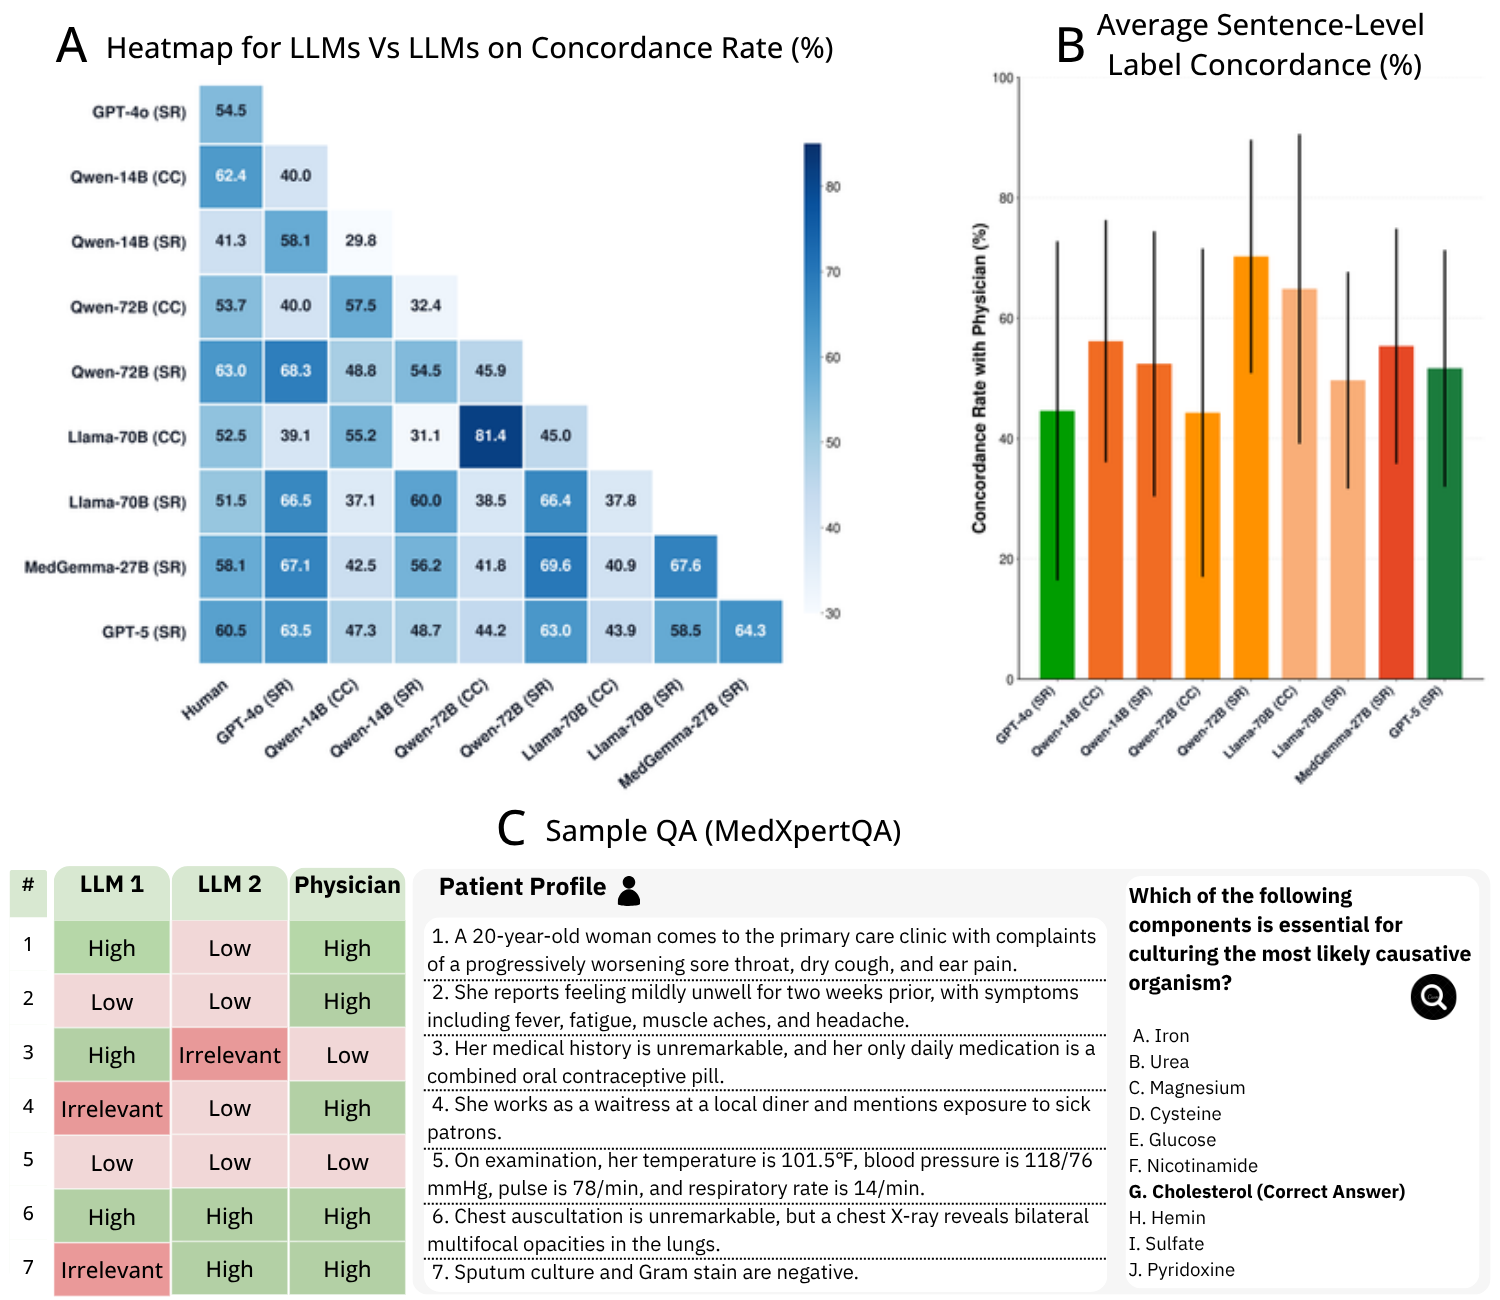
\includegraphics[width=\textwidth]{Figures/Concord_Rate_Sample.png}
  \caption{\textbf{Average Sentence-Level Label Concordance}. Panel A shows the sentence-level concordance between physician trainees and LLMs, as well as between the various LLMs studied. This concordance is highly variable across different LLMs. ``CC'' denotes that the comparison uses ContextCite score and ``SR'' denotes that it uses self-reported labels. Panel B shows a sample item from MedXpertQA. Panel C shows ....}
  \label{concordance}
\end{figure}

The best performing model, Llama-70B, reaches a mean agreement of 65.9\% with the physician trainees, which is below the 72.0\% rate of expert physician agreement but not dramatically so. Overall, roughly one-third of sentences that physician trainees consider highly relevant are not regarded as highly relevant by at least one of the models (Figure~\ref{concordance}).


A common pattern noted in these disagreements is over-attention to superficial cues in the LLM ratings. For example, a model might latch onto a laboratory value that is extreme and assume it must be important, even if it is not relevant to the question at hand. %In one case, an LLM fixated on an incidental finding (“mild elevation in liver enzymes”) when diagnosing a skin rash, marking that sentence as relevant and incorporating it into its answer explanation – a form of distractor usage. The human annotators, by contrast, recognized that the rash diagnosis had nothing to do with the liver enzyme quirk and flagged that sentence as irrelevant. Such cases reveal how an LLM’s internal heuristics (e.g. “unusual values are important”) can mislead its reasoning, whereas human experts apply informed judgment to filter out red herrings. 
Conversely, models sometimes missed subtle but crucial cues that humans tagged as relevant. %For instance, a single sentence mentioning “\textit{recent travel to the Ohio River Valley}” in a patient’s history is a critical clue for a fungal infection diagnosis, physician labelers spot it immediately as a key piece of context, but a LLM might ignore it if it hasn’t connected that region with certain infections in its knowledge. These misses show that even highly knowledgeable LLMs may fail to connect the dots in context, especially when the clue requires integrating world knowledge in a non-obvious way.
These findings could be partially due to LLMs attributing incorrect answers on misinterpreted or irrelevant context, indicating flawed input context relevance estimates. ContextCite highlights cases where a model justifies its answer by citing a sentence it wrongly deems supportive, a phenomenon that researchers call contributive attribution. %For instance, a model might recommend an inappropriate treatment due to a misread clinical detail. These discrepancies between model-perceived and expert-validated relevance expose critical gaps in reasoning.

%By surfacing such divergences, \emph{MedPAIR} pinpoints where models over-rely on spurious cues or fail to distinguish key from peripheral information. These insights offer actionable targets for refining models or prompts, such as encouraging more deliberate evidence selection or filtering superficial correlations.

% \begin{table}[]
% \begin{tabular}{l|ll|ll|l}
% \toprule
%  & \multicolumn{2}{c|}{Self-Report} & \multicolumn{2}{c|}{ContextCite} & Spurious Factors \\
%  \midrule
% Data Source & \begin{tabular}[c]{@{}l@{}}Recall \\ (TPR)\end{tabular} & Kendall $\tau$ & \begin{tabular}[c]{@{}l@{}}Recall \\ (TPR)\end{tabular} & Kendall $\tau$ &  \\
% \midrule
% MMLU &  &  &  &  &  \\
% JAMA &  &  &  &  &  \\
% MedBullets &  &  &  &  &  \\
% MedXpertQA &  &  &  &  &  \\ \hline
% Overall &  &  &  &  & \\
% \bottomrule
% \end{tabular}
% \caption{\textbf{Data Analysis.} TPR indicates True Positive Rate.}
% \label{Confusion_Matrix}
% \end{table}

% \begin{table}[h!]
% \centering
% \resizebox{\textwidth}{!}{%
% \begin{tabular}{l|cc|cc|cc|cc|cc}
% \toprule
% & \multicolumn{2}{c|}{\makecell[c]{MMLU \\ Precision Medicine \\ (250 QAs)}} 
% & \multicolumn{2}{c|}{\makecell[c]{JAMA \\ Clinical Challenge \\ (750 QAs)}} 
% & \multicolumn{2}{c|}{\makecell[c]{Med Bullets \\ (250 QAs)}} 
% & \multicolumn{2}{c|}{\makecell[c]{MedXpertQA \\ (750 QAs)}} 
% & \multicolumn{2}{c}{\textbf{\makecell[c]{Overall \\ (2000 QAs)}}} \\
% \midrule
% & Before & After & Before & After & Before & After & Before & After & Before & After \\
% \midrule
% Qwen-14B     & Acc \% [Std] & -- & -- & -- & -- & -- & -- & -- & -- & -- \\
% GPT-4o     & 1.00 [1.69] & 0.49 [0.85] & 1.75 [2.55] & 0.88 [1.33] & 1.93 [2.09] & 0.94 [1.05] & 1.06 [2.08] & 0.53 [1.05] & 1.42 [2.26] & 0.71 [1.16] \\
% LLaMA-70B    & 77.94\% [0.42] & -- & 48.07\% [0.50] & -- & 48.66\% [0.50] & -- & 14.86\% [0.36] & -- & 30.04\% [0.46] & -- \\
% Qwen-72B    & 89.34\% [0.31] & -- & 57.93\% [0.50] & -- & 62/42\% [0.49] & -- & 16.16\% [0.37] & -- & 35.13\% [0.48] & -- \\
% \bottomrule
% \end{tabular}
% }
% \caption{Number of Irrelevant Sentences}
% \label{tab:comparison}
% \end{table}

% \newpage
% % \section{Sample QA Case Study}
% \label{sample}
% \begin{tcolorbox}[colback=blue!3!white, colframe=blue!50!white, title=Example of QA Data (from MedXpert QA), left=10mm, breakable]
% \small

% \textbf{Patient Profile:} % ++-; +--; -+0; +-0; ---; +++; +-+; FIND HUMAN low/irr but GPT-4o relevant
% \begin{enumerate}
%   \item A 20-year-old woman comes to the primary care clinic with complaints of a progressively worsening sore throat, dry cough, and ear pain.
%   \item She reports feeling mildly unwell for two weeks prior, with symptoms including fever, fatigue, muscle aches, and headache.
%   \item  Her medical history is unremarkable, and her only daily medication is a combined oral contraceptive pill.
%   \item She works as a waitress at a local diner and mentions exposure to sick patrons.
%   \item On examination, her temperature is 101.5℉, blood pressure is 118/76 mmHg, pulse is 78/min, and respiratory rate is 14/min.
%   \item Chest auscultation is unremarkable, but a chest X-ray reveals bilateral multifocal opacities in the lungs.
%   \item Sputum culture and Gram stain are negative.
% \end{enumerate}

% \bigskip
% \textbf{Question: }Which of the following components is essential for culturing the most likely causative organism?


% \bigskip
% \textbf{Options:}
% \begin{enumerate}[label=\Alph*.]
%   \item Iron 
%   ...
%   % \item Urea 
%   % \item Magnesium
%   % \item Cysteine 
%   % \item Glucose 
%   % \item Nicotinamide 
%   % \item Cholesterol  
%   % \item Hemin 
%   % \item Sulfate 
%   \item Pyridoxine
% \end{enumerate}

% \bigskip
% \textbf{Correct Answer:} (G) Cholesterol

% \noindent
% \label{tab:sample_case_label}

% \medskip
% \centering
% \setlength{\tabcolsep}{4pt}
% \begin{tabular}{|l|l|l|l|}
%   \toprule
%   Sentence \# & Physician Labels & GPT4o Self-Reported Labels & MedGemma-27B Labels \\
%   \midrule
%   1 & High & High & Low\\
%   2 & High  & Low  & Low\\
%   3 & Low  & High & Irr\\
%   4 & High  & Irr  & Low \\  
%   5 & Low  & Low  & Low\\
%   6 & High  & High & High\\
%   7 & High  & Irr  & High \\    
%   \bottomrule         
% \end{tabular}
% \end{tcolorbox}


\subsection{Filtering for Human-labeled Relevance Improves LLM Performance (RQ2)}
% We find that MORE HERE ON HOW MODELS ARE BETTER WHEN THEY USE HUMAN RELEVANCE BUT NOT LLM OR CONTEXTCITE?

In accordance with RQ2, we examine the effects of restricting models to using only the sentences that physician trainees have identified as relevant. Removing the sentences that physician trainees marked as low-relevance or irrelevant raises accuracy for most of the LLMs on most datasets (Figure~\ref{results}).

\begin{figure}[h!]
  \centering
  \includegraphics[width=\textwidth]{Figures/MedPAIR_Result_ExpertQA.pdf}
  \caption{\textbf{Effect of Filtering Context on Final Performance.} Figure illustrates how accuracy shifts on four medical benchmarks (MMLU, JAMA, MedXpert, MedBullets) when utilizing various sets of LLMs-labeled highly relevant sentences. Solid black horizontal lines denote the original baseline accuracy, while dotted lines represent the highest accuracy achieved. Colored shapes indicate performance when specific models (GPT-4o, GPT-5, Qwen-14B and Qwen-72B, Llama-70B, MedGemma-27B, Trainee, Physician) highly-relevant sentences are used in predictions. Percentage annotations highlight the largest improvement or decline between the baseline and the best observed accuracy.}
  \label{results}
\end{figure}

We report these accuracy improvements after filtering as observed differences rather than as statistically tested effects. The Round 2 subset contains only 248 QA pairs, so we do not attach confidence intervals or significance tests to the per-dataset changes. Qwen-72B's accuracy rises from 89.3\% to 92.2\% on MMLU Precision Medicine and from 35.1\% to 62.2\% overall, while GPT-4o moves from 39.3\% to 73.0\% overall, keeping its position as the highest performing model before and after filtering. Qwen-14B and Llama-70B show small declines on the MMLU subset (marked in red), which is consistent with sensitivity to small input perturbations in weaker models. Large relative gains for MedGemma-27B are driven by low baseline accuracies and should be interpreted with caution: a change from a low baseline to a still moderate accuracy produces a large percentage change that is not necessarily clinically meaningful. Comparisons with physician trainee unfiltered accuracy (48.3\%) are descriptive; the trainees and the models receive different inputs in the filtered condition and direct head to head claims about clinical parity are not supported by this simplified QA-based design.


% \pgfplotstableset{
%   heatmap/.style={
%     color cells={
%       min=-16.9,
%       max=24.8,
%       textcolor=black,
%       colormap/blues
%     },
%     every head row/.style={before row=\toprule, after row=\midrule},
%     every last row/.style={after row=\bottomrule}
%   }
% }


One interpretation of these results could be that focusing on sentences that physician trainees regard as highly relevant reduces the influence of peripheral content in the LLM output. However, alternative interpretations are equally compatible with the data. Shorter inputs (after removing sentences) are easier for LLMs to process; filtering can incidentally remove adversarial distractors that USMLE-style items include in the questions by design; and especially for older datasets such as MMLU Precision Medicine (released 2020) the filtered input may disrupt patterns associated with memorization. Disentangling these mechanisms is beyond the scope of this study. It is also notable that between 5.8\% and 24.8\% of originally correct predictions flip to incorrect after removing the sentences that physician trainees labeled as low-relevance or irrelevant (Figure~\ref{spurious_info}). Among the LLMs evaluated, Qwen-14B shows the highest \ourmetric and GPT-4o the lowest, with the caveat that this metric is not adjusted for the random-sentence removal baseline for each LLM and may reflect general sensitivity to input perturbation.


% \begin{table}[b]
%   \centering
%   % \renewcommand{\arraystretch}{1.4} 
%   \setlength{\tabcolsep}{10pt} 
%   \begin{tabular}{l@{\hspace{12pt}}|@{\hspace{10pt}}c@{\hspace{15pt}}|@{\hspace{10pt}}c@{\hspace{15pt}}|@{\hspace{10pt}}c@{\hspace{15pt}}|@{\hspace{10pt}}c@{\hspace{15pt}}|@{\hspace{15pt}}c@{\hspace{15pt}}|@{\hspace{15pt}}c}
%     \toprule 
%     \textbf{LLMs} & \textbf{MMLU} & \textbf{JAMA} 
%       & \textbf{MedBullets} & \textbf{MedXpertQA} & \textbf{Total}  & \textbf{Round1 Correct QAs}\\
%     \midrule
%     Llama-70B   & 3.9 & 15.1 & 22.6 & 11.6 & 12.8 & 812\\
%     Qwen-72B    & 2.6  & 8.6  & 5.8  & 4.1  & X & 456\\
%     Qwen-14B    & 9.8  & 13.9 & 18.5 & 8.8 & X & 342 \\
%     MedGemma-27B   & 2.0	& 14.5	& 12.3	& 9.1	& 10.7 & 694\\
%     GPT-4o      & 2.1  & 8.3  & 11.1  & 16.3 & 7.2 & 511\\
%     GPT-5       & 1.1  & 6.6  & 10.5 & 3.1 & 6.0 & 1118\\
%     % Physician   & XX  & XX  & XX & XX \\
%     \bottomrule
%   \end{tabular}
%   \vspace{2mm}
%   \caption{\textbf{The \ourmetric(\%) of removing physician trainee-identified low-relevance and irrelevant sentences.} Each number denotes the proportion of questions that were answered correctly in Round 1 but became incorrect in Round 2 after those sentences were removed.}
%   \label{tab:spurious_rate}
% \end{table}

\begin{figure}[h!]
  \centering
  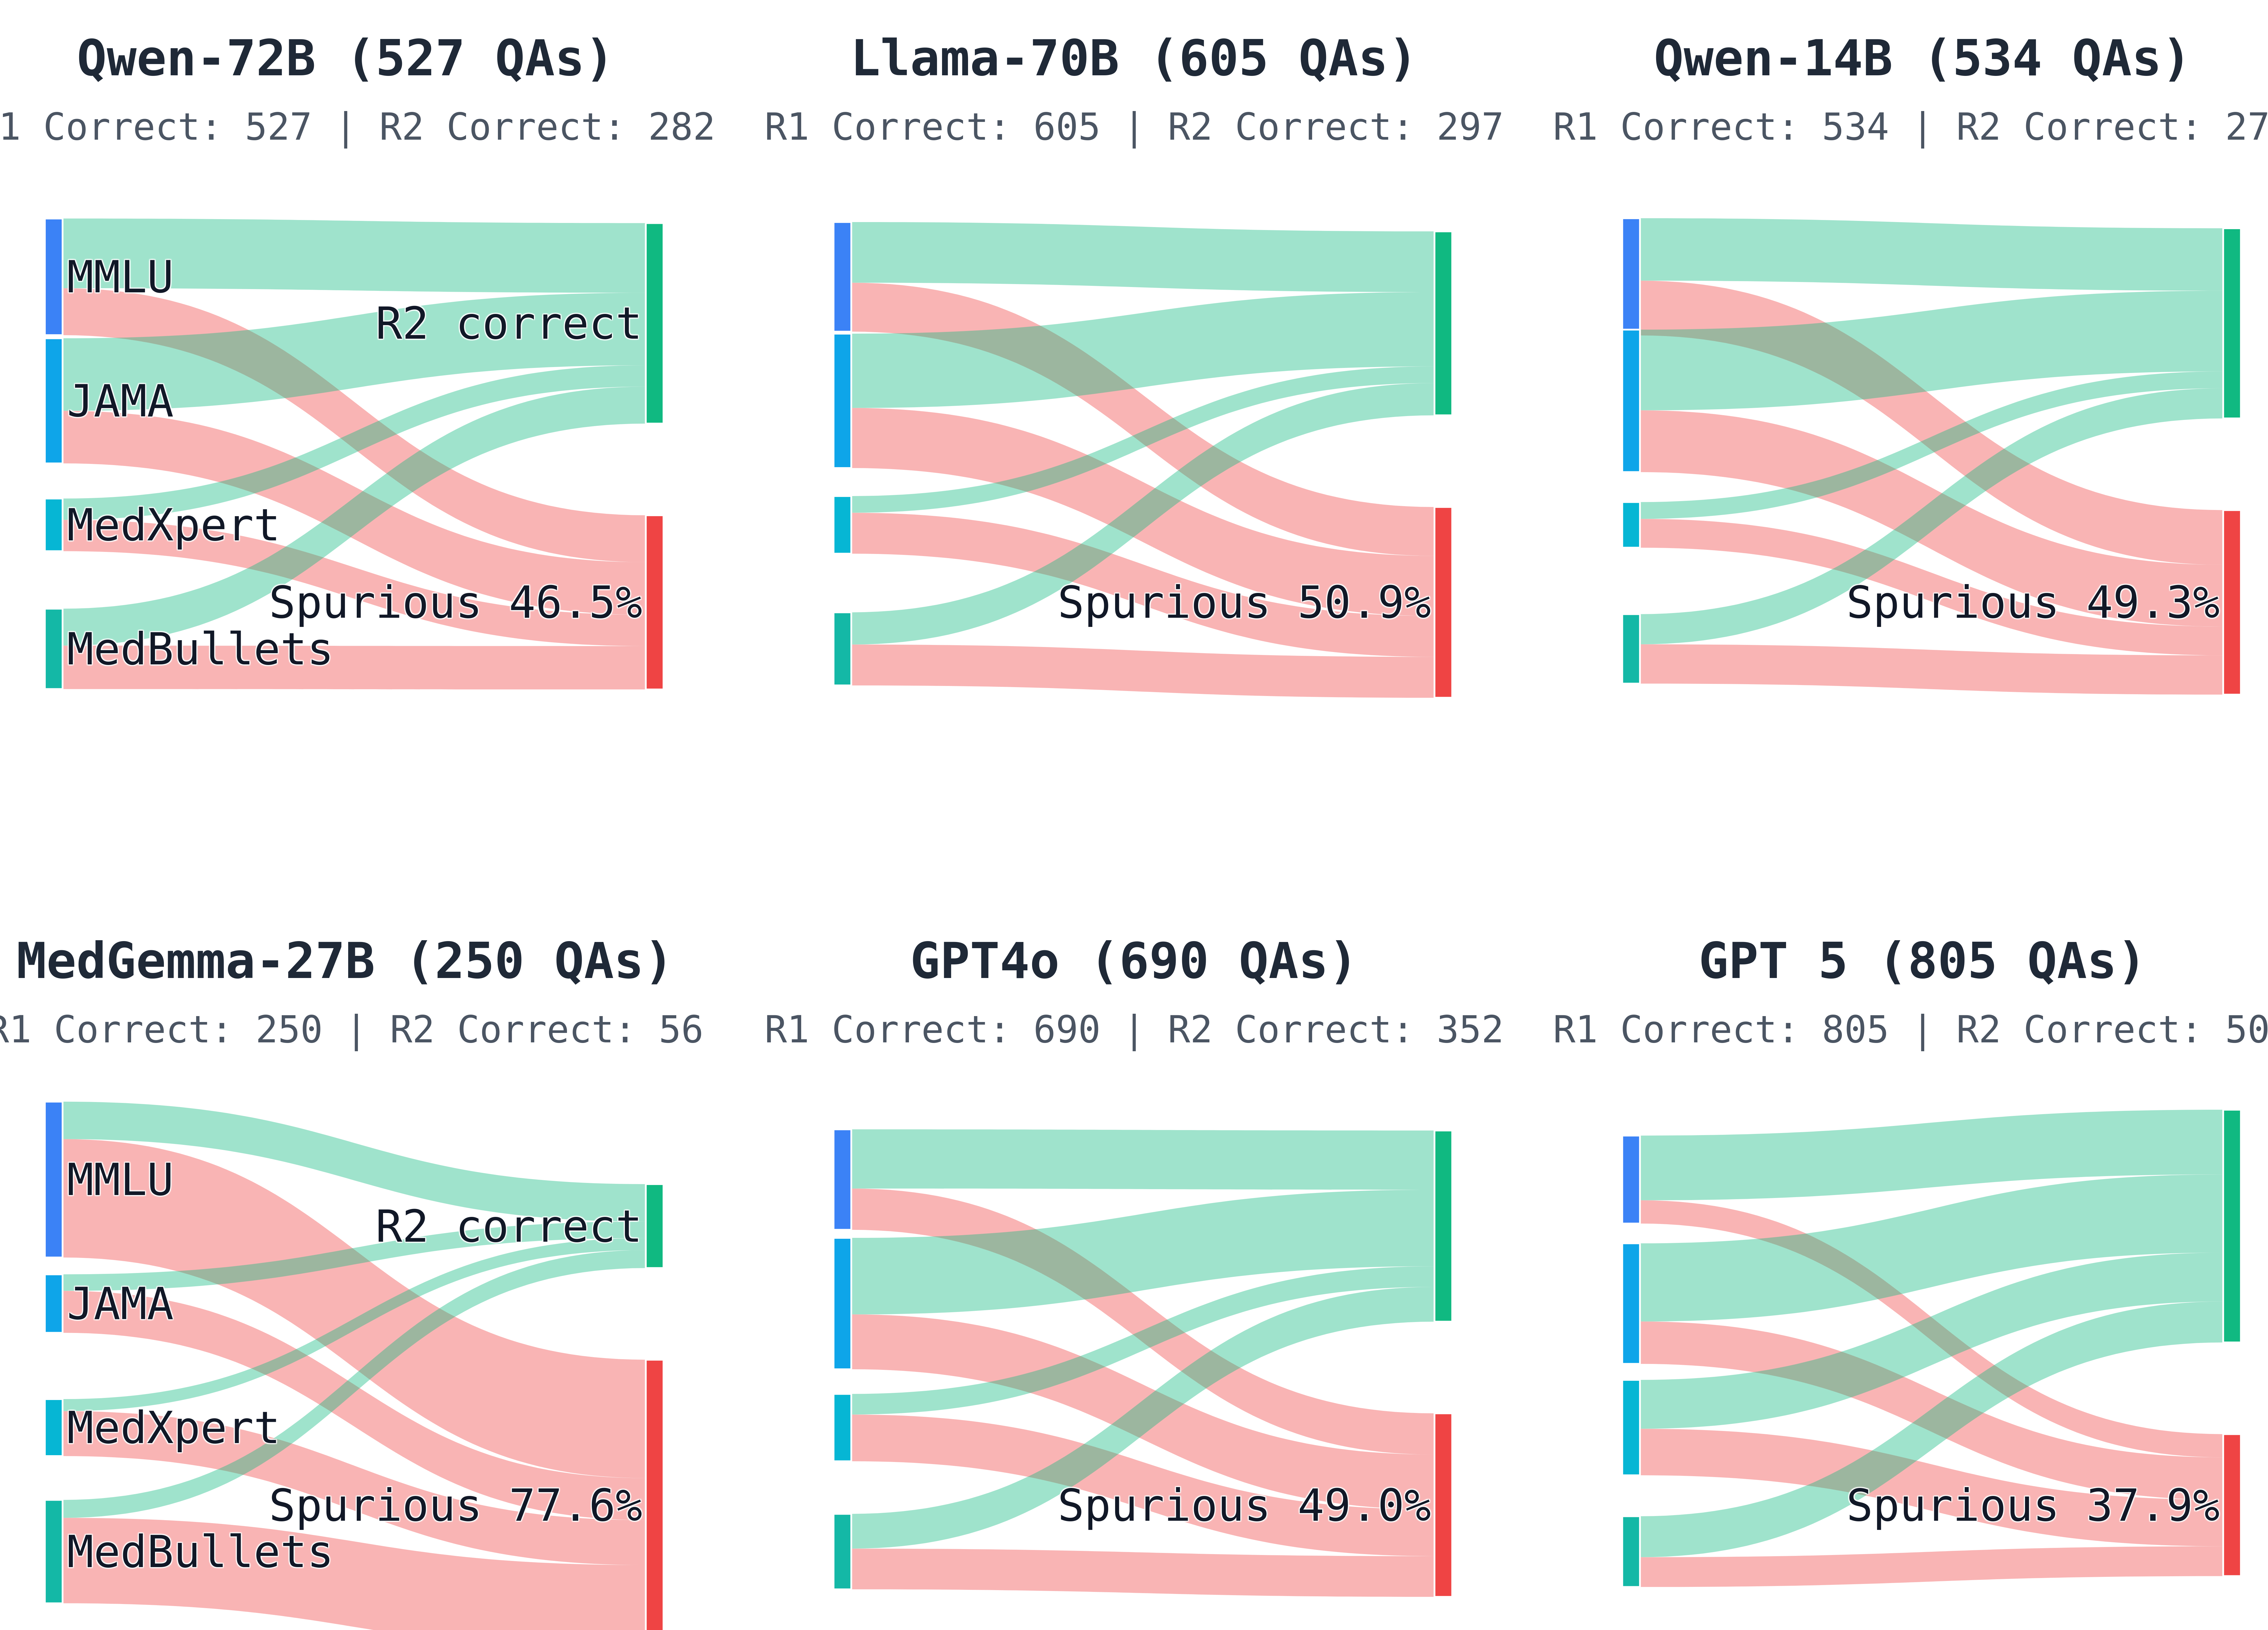
\includegraphics[width=\textwidth]{Figures/llm_sankey_all_models_without_physician.png} % llm_performance_analysis.pdf
  \caption{\textbf{The \ourmetric(\%) of removing physician trainee-identified low-relevance and irrelevant sentences.} The green bars indicate QAs that are correct in the first round and remain correct in the second round, while the red bars indicate the proportion of correct QAs that become incorrect in the second round. These QAs show the opposite trajectory of the intended effect; when low-relevance information is removed the LLM performance for these items deteriorates. For all models, however, the spurious rate is overshadowed by the number of items that change from incorrect in the first round to correct in the second round.} %Among all the models, Qwen-14B varied the most and GPT-5 varied the least.
  \label{spurious_info}
\end{figure}

\subsection{Filtering for LLM-labeled Relevance Can Improve LLM Performance (RQ3)}
%The disagreement between physician trainees and LLMs on input context relevancy reveals differences in how models identify clinically important information.
Since physician trainee annotations are not practical to obtain for every deployment, we next ask if each LLM can select its own relevant sentences in a two-stage process with a similar directional effect. We evaluate task accuracy when each model is restricted to the sentences that it has labeled highly relevant, using per-sentence ContextCite scores from MedGemma-27B, Llama-70B, Qwen-14B, and Qwen-72B, and self-reported labels from GPT-4o and GPT-5. The self-filtering conditions are reported alongside the physician trainee filtering conditions in Figure~\ref{results}.

The most recent flagship LLMs show limited sensitivity to this self-filtering. GPT-5 exhibits almost no change across the four source datasets, while GPT-4o and the Qwen models show small accuracy increases. However, weaker and domain-specialized models have larger relative changes (as noted above, large relative changes from low baselines should be read with caution). Similar directional patterns appear when one model is used to filter another model's input. We do not claim that self-filtering produces a new, higher performance regime; the more conservative reading is that input restriction based on a model's own attribution scores is not systematically harmful and can yield small gains on several benchmarks.

At the dataset level, JAMA Clinical Challenge is the most difficult benchmark for all models, with accuracy between 3\% and 33\%, and with only modest improvements from relevance-based filtering. These observations suggest that part of the gap between weaker and stronger models on \emph{MedPAIR} is associated with how much each model is distracted by content that is not decisive for the question, although the effect is not large enough to overturn the existing model ordering.

\section{Discussion}

Our findings point to a moderate but consistent gap between the relevance judgments of physician trainees and those of current LLMs on clinical QA vignettes, with LLM concordance of 44.9\% to 65.9\%, compared against a board-certified physician accordance of 72.0\% with the trainees. These findings resonate with earlier work showing that LLM performance can be overestimated when benchmark accuracy is read in isolation \cite{bao_llms_2024, ishii_analysis_2024, de2024text}. We interpret our results as evidence that accuracy metrics alone do not fully describe how LLMs arrive at their answers in this setting, rather than as a sharp dichotomy between aligned humans and misaligned models.

Better alignment between LLM-selected and clinician-selected evidence is a plausible ingredient of clinically deployable AI \cite{gourabathina2025medperturb}, but our study does not directly measure clinical deployment outcomes. Our items are multiple-choice exam questions, and the sentences labeled as irrelevant in USMLE-style vignettes often serve a pedagogical purpose. Real clinical notes contain redundant, noisy, and sometimes contradictory content drawn from different distributions. Readers should therefore treat our findings as an evaluation study that informs the interpretation of existing medical QA results, and not as direct evidence about behavior in live clinical workflows \cite{yang_harnessing_2023}.

Previous work has shown that selectively pruning input contexts and retaining only the most relevant content can improve QA performance in language models \cite{mckechnie_context_2025, kabongo_effective_2024}. Our analyses extend these findings to the clinical QA setting by showing that physician trainee annotated context reduction, ContextCite scores from open-source models, and self-report prompting of closed-source models all produce directional accuracy gains across four medical QA datasets. The \emph{MedPAIR} dataset makes this kind of analysis possible by pairing sentence-level relevance labels from physician trainees with LLM-derived labels on the same items, and we release it so that subsequent studies can revisit reasoning patterns in medical LLMs without recollecting expert annotations.

The empirical findings also speak to whether an LLM can take the place of a human annotator in relevance labeling. While self-reported and ContextCite labels exhibited moderate agreement with physician trainees, the observed gaps and the larger accuracy gains obtained with physician trainee filtering indicate that expert oversight remains valuable in this evaluation setting \cite{shi_judging_2025, zheng_judging_2023, soboroff_dont_2025, qiu2025quantifying}. The previously established sensitivity of ContextCite and self-reported labels to prompt and scoring choices, especially in healthcare, suggests that LLM-generated relevance labels should be used alongside, rather than in place of, human annotations when model outputs carry clinical consequences \cite{li2025medguide, abbasiantaeb_can_2024}.

% Interpreting LLM's input relevance scoring using ContextCite scores and self-reported labels may lack reliability. ContextCite scores do not necessarily reflect the clinical relevance of individual sentences in medical question answering, as it designed primarily for context attribution rather than explicit relevance evaluation. Also, self-generated relevance labels by LLMs can be inconsistent or prone to hallucination, often diverging from human expert annotations. Thus, it is essential to systematically investigate how LLMs determine sentence-level relevance in patient profiles and develop dedicated evaluation metrics that accurately capture the nuances of clinical relevance in these contexts.

% Our ultimate goal extends beyond structured and standardized QA datasets to enhance the ability of LLMs to accurately interpret and process medical information across diverse modalities, such as text, images, audio, and video. As these models become increasingly embedded within complex clinical environments, their capacity to reliably identify, prioritize, and reason about clinically relevant content becomes critical. The \emph{MedPAIR} benchmark offers high-quality, physician-derived relevance annotations, providing valuable insight into physicians' initial reasoning processes. We anticipate this benchmark will support the development of more generalizable, interpretable, and trustworthy reasoning across diverse biomedical applications.

% Some recent works on self-critique or chain-of-thought verification might allow an LLM to internally ask itself if it used all relevant info, mimicking what we did externally. Another limitation is that our evaluation of reasoning alignment focused on explicit mentions in the chain-of-thought. It’s possible the model “implicitly” used a clue without stating it. We tried to mitigate this by examining whether excluding a detail caused wrong answers (a proxy for whether it was used), but there’s still some ambiguity. Future research could use more sophisticated methods like input perturbation tests: remove or alter a supposedly relevant detail and see if the model’s answer changes. This would directly test faithfulness: did that detail truly drive the answer? Such analyses complement our approach and could be integrated to validate model reasoning.

% \section{Limitation \& Future Work}

% While our intervention improved alignment, it is a simplified setup. We had the luxury of human annotations for each question, which is not available in real time for novel cases. In practice, one might deploy a two-step system: first have the model or another auxiliary model predict what parts of a case are relevant (perhaps via a model trained on our annotated data), then feed those to the main model. This could approximate our guided approach without needing a human in the loop every time. 

This study has several limitations that future work should address. The human reference in our downstream analyses is a majority vote of physician trainees rather than independent attending physicians, and the 72.0\% trainee--physician matching rate establishes an agreement ceiling that should be kept in mind when interpreting the LLM concordance numbers. We did not separately estimate inter-trainee reliability with standard agreement statistics such as Fleiss' kappa or Krippendorff's alpha, and we treat the trainee majority vote as a pragmatic reference. The ternary High / Low / Irrelevant scheme is coarse by design, and our filtering experiments collapse Low Relevance and Irrelevant into a single removed category even though Low Relevance sentences can still support ruling out alternatives, which is a real diagnostic function. The ternary mapping from continuous ContextCite scores holds the per-item number of high relevance sentences fixed to match the trainee majority vote, so concordance measures ranking agreement are conditional on that count rather than an absolute threshold; we discuss alternative mappings in the Supplementary Information.

Our filtering experiments do not disentangle reductions in distraction from several other potentially confounding mechanisms, including shorter input, disruption of patterns associated with training set memorization on older source datasets such as MMLU Precision Medicine (2020), and incidental removal of adversarial distractors that USMLE-style items include by design. We did not include a matched random sentence-removal baseline, and without this baseline the \ourmetric cannot be uniquely attributed to reliance on content that clinicians would consider peripheral \cite{gu_survey_2025, panickssery_llm_2024, radevski2025synthesizing, zuccon2023chatgpt}. The Round 2 filtering analysis is based on 248 QA pairs and we report observed accuracy differences rather than confidence intervals or significance tests; large relative gains for models with very low baselines, such as MedGemma-27B, should be read in absolute rather than relative terms. The LLMs studied include a mixture of open- and closed-source systems and is not exhaustive---the omission of Med-PaLM, Claude, and other salient models limits the breadth of cross-model comparisons. Finally, the \emph{MedPAIR} dataset is built from multiple-choice exam QA, and the relevance patterns in exam vignettes may differ systematically from those in real clinical notes \cite{croxford_current_2025, sharma_relevance_2017}. In future work \emph{MedPAIR} can support studies with matched random and clinician-varied baselines, contamination audits, finer-grained label schemes, and broader LLM coverage.

%We anticipate this benchmark will support the development of more generalizable, interpretable, and trustworthy reasoning across diverse biomedical applications.

\section{Methods}
% \subsection{Ethical Approval}

% We obtained approval from the MIT Committee on the Use of Humans as Experimental Subjects (IRB: 2504001610) and preregistered our dataset collection protocol on the Open Science Framework (OSF) \cite{hao_alhamoud_jeong_puri_torr_kalantari_schaekermann_stern_ghassemi_2025}. No personally identifiable patient information was involved in this study.

\subsection{Expert Data Annotation}

We partner with Centaur Labs (\url{https://centaur.ai}) to employ board-certified physicians and physician trainees (medical students or higher qualifications) to annotate the QA pairs. Physician trainees are chosen for their familiarity with medical exam preparation, as these questions are primarily designed for medical students. Demographic information for the participants is presented in the Supplementary Information.

A total of 52 physician trainees participated (26.9 years mean age), with 77.3\% at the advanced training level. Among these participants, 67.4\% of the labelers had passed the United States Medical Licensing Examination (USMLE) Step 1 Exam. Notably, half of them reported familiarity with using LLMs in clinical contexts, such as integrating AI tools into clinical queries or workflows. On average, each labeler spent an average of 3.15 minutes (SD 2.90, 95\% CI: 3.04–3.25, n = 2952) per QA. Medical students spent on average 3.19 minutes (SD 3.16, 95\% CI: 3.21-3.44, n of total annotations = 2018); physicians spent on average 3.05 minutes (SD 2.25, 95\% CI: 2.90-3.19, n of total annotations = 934). For each case, the participants first selected the most appropriate answer and then annotated the relevance of every sentence in the patient profile.

A total of 7 physicians participated (43.4 years mean age; 4 reporting as male, 3 reporting as female), with an average of 17.0 years of post-graduate employment. All physicians have passed USMLE Step 3 or equivalent exams. The physician cohort showed high familiarity with the use of LLMs in healthcare, with 5 out of the 7 physicians reporting positive views that LLM deployment is ready for clinician-in-the-loop tasks.

A sample physician trainees' annotation is presented in Figure \ref{fig:study_design} (orange boxes). Full study instructions and the pre- and post-survey instruments are provided in the Supplementary Material. Data collection for the annotations occurred between March 6 and May 5, 2025.

% To avoid spurious correlations from conditioning relevance on known answers, \emph{MedPAIR} collects relevance judgments from physician trainees without disclosing the correct answer and evaluates model performance on held‐out cases, ensuring that any gains reflect genuine improvements in focus and efficiency rather than answer leakage.

Each QA is annotated by at least three physician trainees, and we verify that at least one of the annotators provides the correct answer to the medical question. For each sentence, annotators then apply one of three labels, according to the following instructions: (1) \textbf{High Relevance:} Information that is critical and must be considered to answer the question correctly. These are the key clinical clues or data points that strongly point toward the correct diagnosis or decision. (2) \textbf{Low Relevance:} Information that provides some context or minor clues but is not essential. These details might help rule out alternatives, yet the question could still be answered correctly without them. (3) \textbf{Irrelevant:} Information that is not pertinent to determining the correct answer. These can be distractors or background details included in the vignette that do not impact the outcome in the given context.

This level of detailed expert labeling is largely absent from existing medical QA benchmarks, which typically include only the question and answer, without explicit identification of supporting case details and their degree of relevance \cite{chen_benchmarking_2025}.

\subsection{LLM Data Annotations}

We access the closed-source models (OpenAI) through their respective Python API libraries from March to October 2025. For the open-source models (Llama, Qwen, and Meditron), we employ the Hugging Face Transformers library. These models are executed on a local cluster equipped with four NVIDIA A100 GPUs (80 GB each). All models run with default hyperparameters.

To directly compare the majority-vote annotations of the physician trainees with the labels generated by LLM for each QA, we annotate the LLM outputs using ContextCite for open-source models and using a self-report prompt for all models. ContextCite scores approximate the model's attention distribution \cite{bohnet_attributed_2023}.

ContextCite provides a simple, scalable mechanism for tracing portions of a generated response back to specific input sentences \cite{cohen-wang_contextcite_2024}. For the self-reported outcomes, we proceed in the same manner as the physician trainee labeling protocol: we feed the identical instruction prompt three times into the LLM and determine the relevance label for each sentence by majority vote. Each model receives the identical instruction prompt used by the physician labelers. The complete prompts for generating self-reported labels and ContextCite annotations are provided in the Supplementary Information.

\subsection{Problem Formulation}

Suppose that a particular question consists of a set of sentences $\mathcal{S} = \mathcal{S}^+ \cup \mathcal{S}^-$, where $\mathcal{S}^+$ is the set of relevant sentences (as labeled by a physician trainee), and $\mathcal{S}^-$ is the set of irrelevant sentences. Let $Y \in \{1, 2, ..., K\}$ be the true label. Suppose we have some LLM $f: 2^{\mathcal{S}} \rightarrow \{1, 2, ..., K\}$.

To evaluate if $f$ answers the question using the same information as a human, we compare $f(\mathcal{S})$ with $f(\mathcal{S}^+)$, under the assumption that the set $f(\mathcal{S}^+)$ is sufficient for a human to answer the question correctly. This gives us the following possible scenarios:
\begin{enumerate}
 \item $f(\mathcal{S}) = f(\mathcal{S}^+) = Y$: The model is correct in both cases, suggesting that it relies on the same information as a human to solve the problem.
    \item $f(\mathcal{S}) \neq Y,  f(\mathcal{S}^+) \neq Y$: The model is incorrect in both cases, indicating that the problem is inherently difficult or $f$ has poor capabilities.
     \item $f(\mathcal{S}) = Y,  f(\mathcal{S}^+) \neq Y$: By removing irrelevant sentences, we flip a correct prediction to an incorrect one. This indicates that the model may have been relying on spurious information in $\mathcal{S}^-$ (i.e. information for which a human deems irrelevant) to make its predictions. 
      \item $f(\mathcal{S}) \neq Y, f(\mathcal{S}^+) = Y$: The model improves when irrelevant information is removed, indicating that $\mathcal{S}^+$ contains sufficient information to answer the question as expected, and the presence of $\mathcal{S}^-$ introduces noise or distractions.
\end{enumerate}

As case (3) is the most salient for our purpose, we define the \ourmetric (\textbf{S}purious \textbf{R}ate) as the prevalence of samples in this case:
$$\ourmetric(f) = \frac{\sum_{i=1}^N \mathbf{1}[f(\mathcal{S}_i) = Y_i \land f(\mathcal{S}_i^+) \neq Y_i]}{\sum_{i=1}^N \mathbf{1}[f(\mathcal{S}_i) = Y_i]},$$
where $N$ is the total number of questions. We treat \ourmetric as a proxy rather than a direct measure of spurious reasoning. Removing sentences changes the input distribution, and any model may behave differently on a truncated input regardless of whether or not the removed content is informative. The physician trainee labels that define $\mathcal{S}^-$ are themselves noisy, so the metric also reflects sensitivity to label noise. A fully controlled interpretation would require a random sentence-removal baseline matched for length, which we leave to future work. With these caveats in mind, a higher \ourmetric indicates that more of a model's originally correct answers do not survive the removal of sentences that physician trainees judge as low-relevance or irrelevant, while a lower value indicates more robustness to this particular perturbation.

\section{Data Availability}
All data underlying this study’s results are provided in the Supplementary Data. All LLM and physician trainee-labeled data are available at: \url{http://medpair.csail.mit.edu/}. The physician trainee-annotated data are available to use through HuggingFace at \url{https://huggingface.co/datasets/YuexingHao/MedPAIR}.

\section{Code Availability}
All code used in generating this study's results is presented in the Supplementary Data.

\section{Acknowledgements}
This work was supported in part by an award from the Hasso Plattner Foundation, a National Science Foundation (NSF) CAREER Award (\#2339381), and an AI2050 Early Career Fellowship (G-25-68042). We also thank Morgan Bouie and Susan Campbell at Centaur Labs for their efforts in coordinating the physician trainees’ data annotations, and Walter Gerych and Olawale Salaudeen for their valuable feedback that strengthened this manuscript.

\section{Author Contributions}

Y.H., K.A., H.Z., and M.G. conceived and designed the study. Y.H., K.A., G.Y., and H.J. carried out data collection, processing, and experimental analysis. H.Z., G.Y., I.P., P.T., M.S., S.K., and A.D.S. offered critical intellectual input and guidance. Y.H., H.Z., H.J., and M.G. drafted the initial version of the manuscript. M.G. secured funding and provided overall supervision. All authors contributed to administrative, technical, and material support, reflecting a comprehensive and collaborative team effort.

\section{Competing Interests}
The authors declare that they have no competing interests.


\bibliography{references}

\end{document}